\documentclass[11pt, a4paper, twoside]{Thesis}
\usepackage{etex}
%\usepackage{arabtex}
%\usepackage{utf8}

\usepackage{subcaption} % not
%\usepackage{amsmath}
\usepackage{tocbibind}
%\usepackage{packages/algorithm2e}
\usepackage{multirow}
\usepackage{setspace}
\usepackage{tikz} % not
\usetikzlibrary{shapes.geometric, arrows}
\usepackage{microtype}
\usepackage{makeidx}
\makeindex


\usepackage{standalone}
\usepackage{tabularx} % not

\usepackage{tikz}
\usepackage{tikz-qtree}
\usetikzlibrary{trees} % this is to allow the fork right path
% \usepackage{dirtytalk}
\usepackage{float}


\newcolumntype{Y}{>{\centering\arraybackslash}X}

\setlength{\parindent}{0.7cm}

\makeatletter
\DeclareRobustCommand\onedot{\futurelet\@let@token\@onedot}
\def\@onedot{\ifx\@let@token.\else.\null\fi\xspace}



\def\eg{\emph{e.g}\onedot} \def\Eg{\emph{E.g}\onedot}
\def\ie{\emph{i.e}\onedot} \def\Ie{\emph{I.e}\onedot}
\def\cf{\emph{c.f}\onedot} \def\Cf{\emph{C.f}\onedot}
\def\etc{\emph{etc}\onedot} \def\vs{\emph{vs}\onedot}
\def\wrt{w.r.t\onedot} \def\dof{d.o.f\onedot}
\def\etal{\emph{et al}\onedot}
\usepackage[group-separator={,}]{siunitx}

\makeatother

\newcommand{\argmax}{\operatornamewithlimits{argmax}}
\newcommand{\argmin}{\operatornamewithlimits{argmin}}
\newcommand{\abs}[1]{\left\lvert#1\right\rvert}
\newcommand{\norm}[1]{\left\lVert#1\right\rVert}
\newcommand{\listofalgorithmes}{\tocfile{\listalgorithmcfname}{loa}}
\newcommand\Chapter[2]{
  \chapter[#1: {\itshape#2}]{#1\\[1ex]\Large#2}
}

\begin{document}
%\setcode{utf8}

% *************** Front matter ***************
\frontmatter

\title  {Effects of crosstalk on perceived depth in stereoscopic and automultiscopic displays}

\authors  {\texorpdfstring
            {{Waqar Khan}}
            {Author Name}
            }
\addresses  {\groupname\\\deptname\\\univname}  % Do not change this here, instead these must be set in the "Thesis.cls" file, please look through it instead
%\usdate
\date       {Saarbr\"ucken, \today }
\subject    {}
\keywords   {}

\maketitle

%\newpage
%\mbox{}
%\thispagestyle{empty}
%\newpage

\setstretch{1.3}

\thispagestyle{empty}

\section*{Eidesstattliche Erkl\"{a}rung}
Ich erkl\"{a}re hiermit an Eides Statt, dass ich die vorliegende Arbeit selbstst\"{a}ndig verfasst und keine
anderen als die angegebenen Quellen und Hilfsmittel verwendet habe.

\vspace{0.60cm}
\section*{Statement in Lieu of an Oath}
I hereby confirm that I have written this thesis on my own and that I have not used any other media or
materials than the ones referred to in this thesis.
\vspace{1.5cm}

\section*{Einverst\"{a}ndniserkl\"{a}rung}
Ich bin damit einverstanden, dass meine (bestandene) Arbeit in beiden Versionen in die Bibliothek der
Informatik aufgenommen und damit ver\"{o}ffentlicht wird.

\vspace{0.60cm}
\section*{Declaration of Consent}
I agree to make both versions of my thesis (with a passing grade) accessible to the public by having
them added to the library of the Computer Science Department.
\vspace{3cm}

\begin{flushright}
\noindent Saarbr\"{u}cken, \today
\hfill
Waqar Khan
\end{flushright}

\clearpage  % Declaration ended, now start a new page
%% ----------------------------------------------------------------

\newpage
\mbox{}
\thispagestyle{empty}
\newpage

% The Abstract Page
%!TEX root = Thesis.tex
\addtotoc{Abstract}  % Add the "Abstract" page entry to the Contents
\abstract{
\addtocontents{toc}{\vspace{1em}}  % Add a gap in the Contents, for aesthetics
\emph{Stereoscopic and automultiscopic displays suffer from crosstalk, that is undesired effect which greatly reduces image quality, viewer comfort and distort the perception of depth. Previously, only a limited work has been done on understanding the relation between crosstalk and the perceived depth with respect to stimuli of different nature in stereoscopic displays. To the best of our knowledge, no such work has been done for automultiscopic displays. Moreover, most of the previous work is carried using simple monochromatic scenes. Since the human visual system uses numerous cues other than disparity to estimate the depth of an object in a stereo scene, monochromatic scenes are poor choice for understanding the aforementioned effects. In this work, we perform experiments to better understand the effects that crosstalk might have on the perceived depth of stimuli in both, stereoscopic and automultiscopic displays. In order to obtain an accurate understanding, we perform experiments on rendered stimuli of natural scenes consisting of objects of various geometries. The model for human visual system's depth estimation via disparity as provided by the current literature fails to justify why and how the perceived depth is affected by the crosstalk. Based on the result of our experiments, we propose a modified human visual system's depth estimation model that, while estimating the viewer's observed depth of a stereoscopic stimulus, takes the ghosting in consideration as well. Finally, some improved techniques for compensation of crosstalk in automultiscopic displays are proposed.}
}
\clearpage
%% ----------------------------------------------------------------
\newpage
\mbox{}
\thispagestyle{empty}
\newpage

\setstretch{1.3}  % Reset the line-spacing to 1.3 for body text (if it has changed)

% The Acknowledgements page, for thanking everyone
\acknowledgements{
\addtocontents{toc}{}  % Add a gap in the Contents, for aesthetics    \vspace{1em}
\emph{I would like to express my gratitude to my supervisor Karol Myszkowski for introducing me to this topic, and for his remarks and his engagement through the learning process of this master thesis. Furthermore, I would like to thank Belen Masia for her immense support and guidance without which the thesis would not have been completed. Also, I would like to thank the participants in my experiments, who have willingly shared their precious time. I would like to thank my loved ones, who have supported me throughout entire process, both by keeping me motivated and helping me putting pieces together.}

}
\clearpage  % End of the Acknowledgements
%% ----------------------------------------------------------------
\newpage
\mbox{}
\thispagestyle{empty}
\newpage

\newpage
\mbox{}
\thispagestyle{empty}
\newpage

\setstretch{1}
\begin{spacing}{0.1}
\pagestyle{fancy}
\tableofcontents
\newpage
\listoffigures
\newpage
\listoftables
\newpage
%\listofalgorithmes
\end{spacing}

\clearpage

\setstretch{1.3}
% *************** Main matter ***************
\mainmatter

%!TEX root = ../Thesis.tex
\chapter{Introduction}
\label{chap:intro}

Ever since its commercial introduction to cinema in 1922, the stereoscopic approach to 3D content presentation has waxed and waned in popularity over time. Stereoscopy consists of presenting a different perspective image separately to each eye tricking the Human Visual System\index{HVS} (HVS) to see in 3D on a 2D planer flat screen. Current commercial stereoscopic 3D displays, like any other practical system, are not devoid of imperfections. One of these imperfections known as crosstalk, is the inability to separate the different views completely for each eye. This means that some portion of the light from the image intended for one eye leaks to the other eye (and vice versa) that results in dim copies (ghosts) of the unintended images seen along with the intended images. Crosstalk is present in all commercially available 3D displays (LCD TV's and cinemas) and contributes heavily to the viewer's discomfort in the forms of reduced overall image quality and reduced image contrast. More importantly crosstalk also affects the stereopsis of HVS. Unintended depth edges conflict with the intended depth edges, thereby hindering the proper fusion of the stereo images \cite{tsirlin2012effect}. These conflicts can result in reduced observed depth. Thanks to today's technologically impressive and immensely lucrative 3D movie industry, TV and games, the 3D industry has been seeing a sharp rise in popularity. This increase in popularity has once again motivated researchers to give attention to imperfections in commercial stereoscopy and their effects on viewers. Current methods for crosstalk compensation or `deghosting' typically involve subtracting the unintended ghosts from the intended image before being displayed. This technique, however, either reduces the overall image contrast or does not remove the ghosting completely in high contrast regions of the images.


\section{Contribution}

Although the effects of crosstalk on viewer's observed quality and visual discomfort have been thoroughly studied in the past \cite{wilcox2003determinants}, its effects on the depth perception have received little attention. Since the basic purpose of stereoscopy is to display a 3D scene consisting of different objects located at different depths, any undesired variation in the perceived depths can severely hamper the aesthetics of the observed scene. Thus the main focus of this thesis is to better understand the effects that crosstalk can have on the depth perception on various types of images and 3D display technologies. Previously, some  work has been done concluding that crosstalk in general reduces the perceived depth \cite{tsirlin2012effect}, i.e. objects that are distant from the plane of fixation\index{POF} (POF) will tend to fall back to the POF. The user studies that resulted in that conclusion were performed on monochromatic stimuli where disparity was the only cue for depth. The natural scenes usually have a lot more depth cues and hence we hypothesized that the effects of crosstalk might be different for complex stimuli. In order to assess the effects of crosstalk on the viewer's depth perception, we firstly performed experiments on stimuli of various dimensions and shapes that were rendered images of a 3D scene containing all possible depth cues. Further, we found that there have been no studies analyzing the effects of crosstalk on the depth perception in an automultiscopic displays (glass free 3D display). We performed another set of experiments in order to analyze if the effects of crosstalk on depth perception in automultiscopic displays is any different.

We also propose a modified HVS disparity estimation model inspired by the model of Banks et al \cite{filippini2009limits}, that helps understand why the crosstalk results in reduced depth of objects that are located away from the plane of fixation. Finally, we propose and test some new techniques for reducing crosstalk in automultiscopic displays.

\section{Structure}

The thesis is assembled as follows. Chapter 2 discuss some background knowledge required in order to fully understand subsequent chapters. This included information about how the HVS works according to the literature, a formal definition of crosstalk and a general idea of how different 3D displays work along with the nature of their crosstalk. Chapter 3 covers some of the previous research that has been performed in order to understand the effects of crosstalk on perceived depth, the possible explanation for this effect, and different techniques that are used in order to mitigate the effect of crosstalk via image preprocessing. Chapter 4 discusses in detail the experiments we performed to quantify how the depth is degraded in both stereoscopic and automultiscopics screens, along with their results. In Chapter 5, we discuss our proposed modified HVS depth via disparity resolution model that takes the effects of crosstalk into account as well. We also discuss our proposed crosstalk reduction techniques. Finally, in Chapter 6 we will look into some phenomenon that still needs explanation and where the future research could be headed in order to get a better understanding of them.


% \section{List of Commonly used abbreviations}



% \chapter{Background}

\section{Sec1}


\begin{itemize}
\item Definition
\item English NED

\end{itemize}

\section{sec1}
\begin{itemize}
\item test 1
\item test
\end{itemize}

\section{sec2}


section content
%!TEX root = ../Thesis.tex
\chapter{Relevant Background}
\label{chap:reletiveBackground}

Depth perception is the ability of the Human Visual System \index{HVS} to visualize the three dimensional world as well as measuring the distance of an object based on two dimensional images obtained from the eyes. Depth perception is imperative for performing basic everyday tasks such as avoiding obstacles without bumping into them or interacting with the world with relative ease. In animals (specially predators), it is critical to estimate the distance of a prey for an efficient attack. Depth sensation is the term used for animals as it is not known whether they sense the depth in the same way as humans do or not\cite{ wiki:depth_perception}.

% Figure for cues
\begin{figure}
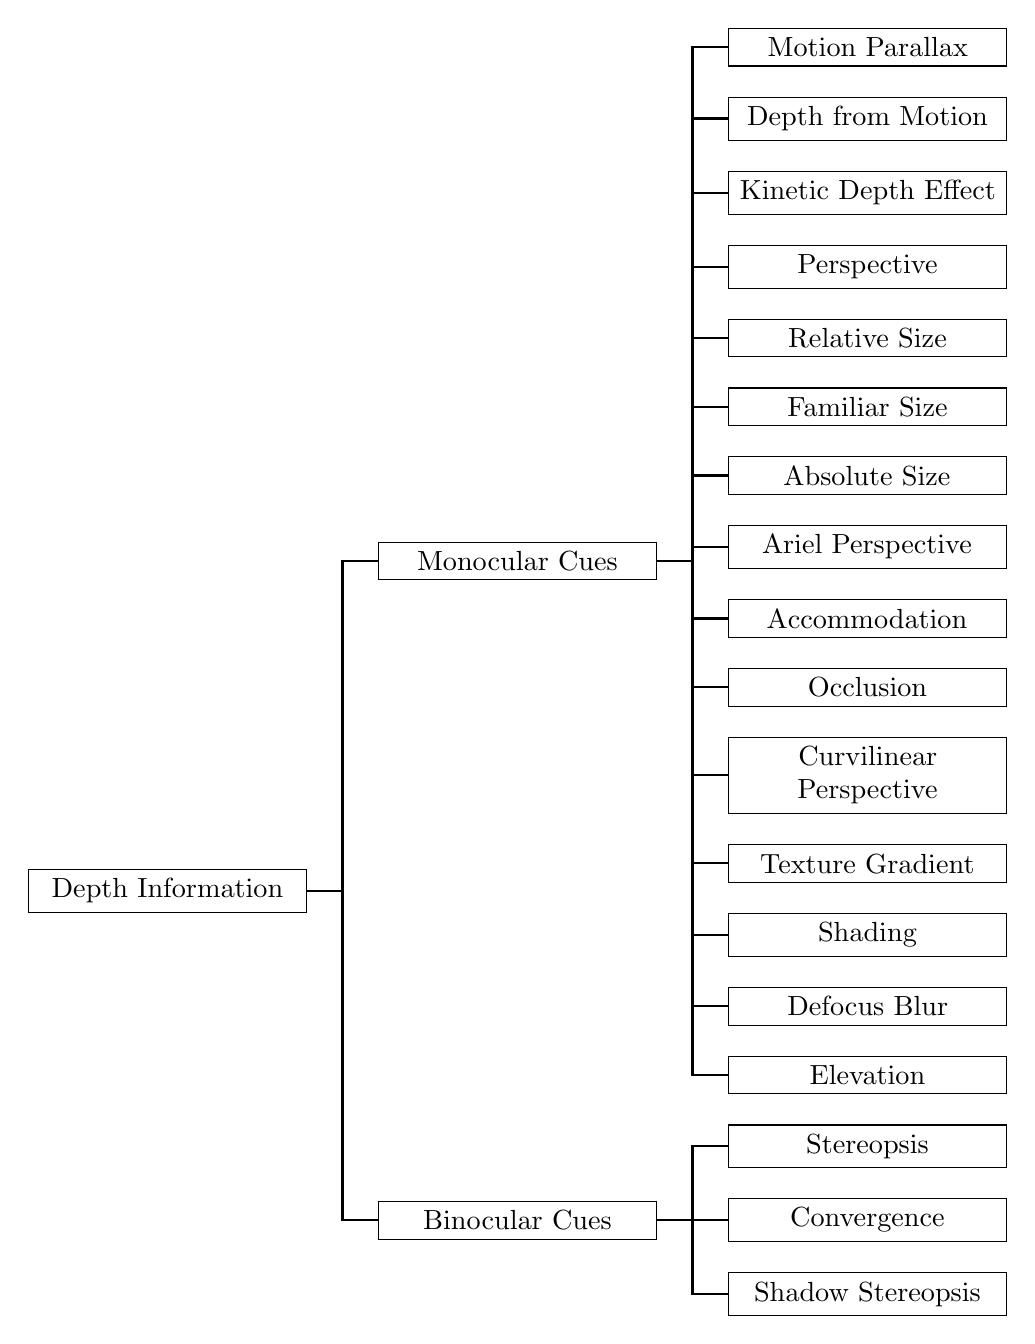
\begin{tikzpicture}[grow'=right,level distance=1.75in,sibling distance=.15in]
\tikzset{edge from parent/.style = {thick, draw, edge from parent fork right},
         every tree node/.style  = {draw,minimum width=1in,text width=1.3in,align=center}}
\Tree
    [. {Depth Information}
	        [.{Monocular Cues}
	                [.{Motion Parallax } ]
	            	[.{Depth from Motion } ]
	            	[.{Kinetic Depth Effect } ]
	            	[.{Perspective } ]
	            	[.{Relative Size} ]
	            	[.{Familiar Size} ]
	            	[.{Absolute Size} ]
	            	[.{Ariel Perspective} ]
	            	[.{Accommodation} ]
	            	[.{Occlusion} ]
	            	[.{Curvilinear Perspective} ]
	            	[.{Texture Gradient} ]
	            	[.{Shading} ]
	            	[.{Defocus Blur} ]
	            	[.{Elevation} ]
	        ]
	        [.{Binocular Cues}
	                [.{Stereopsis } ]
		            [.{Convergence } ]
		            [.{Shadow Stereopsis} ]
	        ]
    ]
\end{tikzpicture}
\caption{HVS Depth Cues\label{fig:CueTree}}
\end{figure}

Human visual system \index{HVS} uses several monocular and binocular cues to determine the depth of objects in the view. These cues can be categorized into two categories i.e. cues extracted from a single image (Monocular Cues) and cues extracted from two images (Binocular cues)\cite{depthcues1}\cite{ wiki:depth_perception}. Figure \ref{fig:CueTree} gives an outlook of the depth cues used by the HVS. These cues are then dynamically weighted according to their robustness by the HVS in order to estimate a depth value for each object in the view \cite{CueFusion}(Write details of those cues in Appendix).


\section{Binocular vision, stereopsis and its limits}
% Limits of stereopsis and that other paper of bank.\cite{banks1}
% cormack paper.
% when fusion and happens and when not and why?
Generally speaking, all the animals with two eyes have binocular vision and they can integrate the information from two eyes based on the binocular overlap. But the term Binocular vision is usually used for the animals that have a large area of binocular overlap (Human and most other predators) and use it to get the depth information of the world around them. In addition to calculating depth, binocular vision also has advantages in performing other tasks such as detection, discrimination, detecting camouflaged objects or eye-hand coordination. Even the resolution observed world is increased with binocular vision\cite{howard1995binocular}. Among all the depth cues discussed in the section above, Stereopsis is the most influential of them all. Since the human eyes are located at different lateral positions on the head, the images formed on the retinas of these two eyes are slightly different. The difference is mainly the horizontal positions of the objects\cite{ wiki:stereopsis}. The process of obtaining a fused (Binocular fusion) image (Cyclopean image) and obtaining a depth map based on the horizontal disparities of the objects in these two images is known as stereopsis.

When the eyes verge in order to focus on some object (or point) in space, that object is projected at identical corresponding points in the retinas. It means that the difference between their horizontal positions is zero. This process is called fixation of the eyes and the distance of the object (point) at which the eyes are fixated is called the fixation distance. The locus of all the points in space that is projected on identical retinal points is called the horoptor\cite{ wiki:horoptor}. Theoretically, via geometrical principles, the horoptor is a circular segment in the plane of fixation point. However, Wheatstone in 1938 observed that the actual/emperical horopter is much larger than that. Figure \ref{fig:horoptor} shows both the theoretical and empirical horoptor. Any object that is farther away from the horoptor has uncrossed disparity in the retinas i.e. the eyes need to be diverged (uncrossed) in order to fixate on that object. Similarly, any object that is closer than the horoptor has crossed disparity in the retinas i.e. the eyes need to be converged (further crossed) in order to fixate at it \textcolor{red}{cite and make the diagram for crossed uncrossed disparities}. Figure ?? shows a graphical representation of crossed and uncrossed disparities \textcolor{red}{add the dolphin images from wikipedia article.}.

\begin{figure}
\centering
    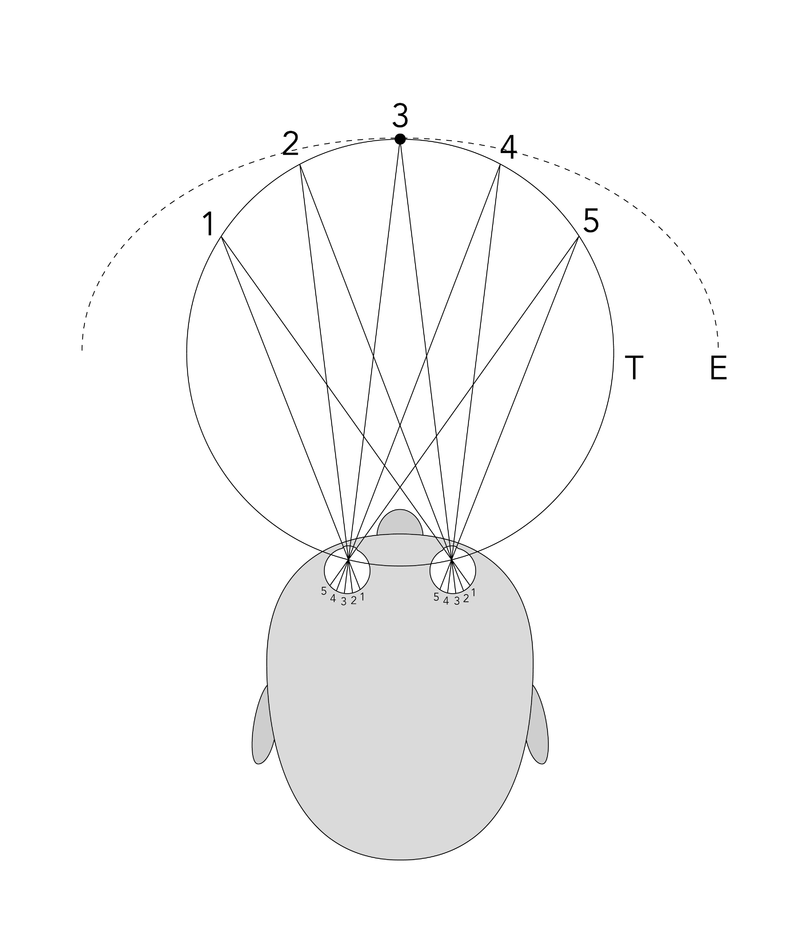
\includegraphics[width=0.5\textwidth]{./Template_Figures/horopter}
    \caption{Representation of theoretical (T) and empirical (E) horoptor\label{fig:horoptor}}
\end{figure}

Stereopsis is believed to be processed in the binocular neurons of the visual cortex of mammals. The binocular neurons have receptive fields in different horizontal positions in each eye. These cells are active only when the object of interest is in certain range of disparity in one eye relative to the other i.e. there is a maximum disparity limit. \textcolor{red}{add the dolphin images from wikipedia article.}. As the objects in the images formed at the retinas of both eyes are slightly shifted horizontally, presenting two different images with shifted object two both eyes can fool the HVS into perceiving depth. This process is called stereoscopy. The first stereoscope was invented by Sir Charles Wheatstone in 1838\cite{ wiki:wheatstone}. It used two mirror both tilted at 45 degrees to the eyes that reflected two different images from the sides. Currently all the stereoscopic screen present a different perspective image two both eyes with different technologies that will be discussed in later sections.

\section{Limits of Stereopsis}
% Limits of stereopsis and that other paper of bank.\cite{banks1}
% cormack paper.
% when fusion and happens and when not and why?
Put it in the section above.








\section{Crosstalk}
% Definitions and Factors contributing to Crosstalk
% Effects on viewers
% 70\% thing etc.
As discussed in the previous section, stereoscopy includes the process of displaying different perspective images to each eye in order to mimic the effect of depth in a scene. However, it is critical that the perspective of these two images should be segregated completely from each other. Currently, all the commercially available 3D displays (with exception of head mounted displays or Wheatstone setups) fail to isolate the two images completely. That means that a percentage of the image of one eye leaks to the other eye as well. This unintended leakage is called the crosstalk in stereoscopic screens\cite{woods2012crosstalk}. Figure \ref{fig:ct1} Shows one such example where the screen has a simulated crosstalk of 14\%. This means that 14\% image intensity of the right eye image is leaked into the left eye image and vice versa.

\begin{figure}[htbp]
    % \centering

    \begin{subfigure}[b]{0.3\textwidth}
        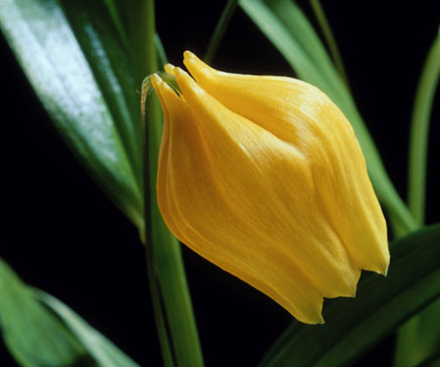
\includegraphics[width=\textwidth]{./Template_Figures/orig}
        \caption{Original Image}\label{fig:originalPicture}
    \end{subfigure}
    \begin{subfigure}[b]{0.3\textwidth}
        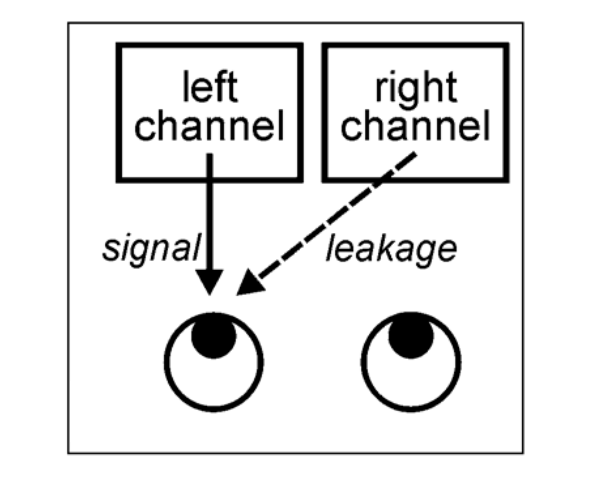
\includegraphics[width=\textwidth]{./Template_Figures/leakage}
        \caption{Original Image}\label{fig:ill_leackage}
    \end{subfigure}
    \begin{subfigure}[b]{0.3\textwidth}
        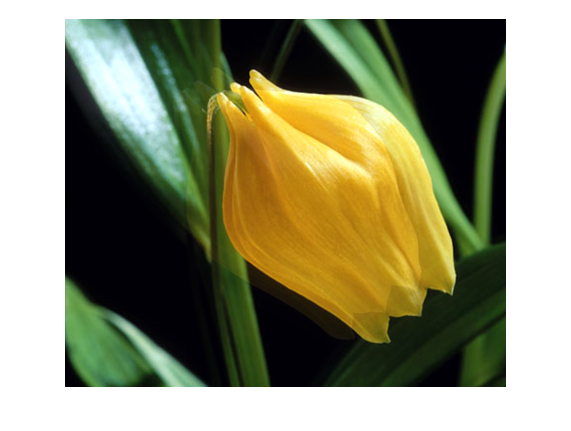
\includegraphics[width=\textwidth]{./Template_Figures/crosstalk}
        \caption{Original Image}\label{fig:imWCT}
    \end{subfigure}

    \begin{subfigure}[b]{0.3\textwidth}
        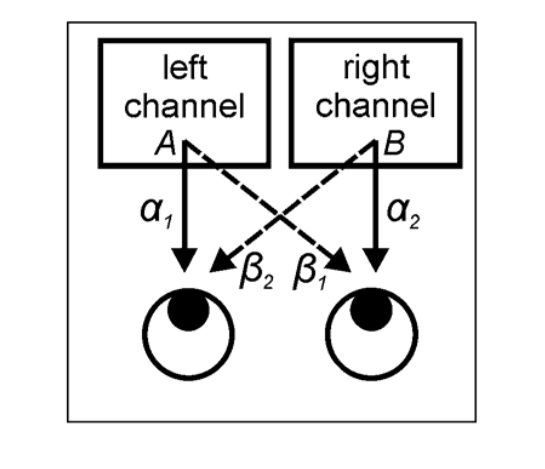
\includegraphics[width=\textwidth]{./Template_Figures/viewerCT}
        \caption{Viewers Crosstalk}\label{fig:viewerCT}
    \end{subfigure}

    \caption{(a-c) A simulation of 14\% crosstalk. An Image intended for the left eye containing 14\% of image intended for right eye. (d) Illustration of Viewers crosstalk with the transfer functions as defined by Andrew J. Woods \cite{woods2012crosstalk} \label{fig:ct1}}
\end{figure}

\say{System crosstalk} is the term used to define the amount of light leakage that occurs between two views and is independent of the image contents. In simplest form, it can be mathematically defined as:

\begin{equation}
Crosstalk(\%) = \frac{leakage}{signal} *100
\label{eq:simple_crosstalk}
\end{equation}

Here, \say{signal} is the luminance of the original image intended for an eye and \say{leakage} is the luminance of the light that leaks from the unintended image. Usually, on a stereoscopic scree, the amount of crosstalk is measured by observing the luminance of the left channel while a black (minimum luminance) image is displayed in the left channel and a white (maximum luminance) image is displayed on the right channel and vice versa. This definition is accurate for the screens that can manage to display a true black i.e. zero luminance. Almost all of the LCDs can not produce zero luminance as their minimum luminance hence resulting in a non-zero black level at its minimum. Another mathematical representation of crosstalk take into effect this non-zero black level and is defined as:

\begin{equation}
Crosstalk(\%) = \frac{leakage - black level}{signal - black level} *100
\label{eq:crosstalk_gray}
\end{equation}

Throughout the rest of the thesis, we will be using crosstalk as mentioned in eq \ref{eq:crosstalk_gray}.

Viewers crosstalk on the other hand is the amount of crosstalk that can be perceived by the viewer as ghosts. It is dependent on the image contents i.e the contrast at the ghosting point and the parallax of objects in the scene. If the system crosstalk is defined as
\begin{equation}
System\ Crosstalk\ (left\ eye) = \frac{\beta_2}{\alpha_1}
\label{eq:system_ct}
\end{equation}

Where \(\alpha_1\) denotes the percentage part of the left-eye image at position (x,y) as observed by the left eye and \(\beta_2\) denotes the percentage amount of right eye image at the same location (x,y) leaked into the left eye. Then the viewers crosstalk is defined as

\begin{equation}
Viewers\ Crosstalk\ (left\ eye) = \frac{B\beta_2}{A\alpha_1}.
\end{equation}

where \say{A} is the luminance of that particular point in left-eye image and \say{B} is the luminance of that particular point in right-eye image (as described in Fig \ref{fig:viewerCT}). The Variables \(\alpha\) and \(\beta\) are characterizing the transfer functions from the displayed image to the observed image i.e. the amount of light reaching the eyes after being displayed on the screen and going through the glasses or any other medium that resides between the screen and the eyes. In most displays, crosstalk is an additive process and is roughly linear. This means that to simulate crosstalk, adding a desired amount of unintended image to an intended image should be sufficient. The simulation of crosstalk in our experiments was carried out in the same manner.

The perception of crosstalk obeys the Webber's law which means that leaked light will be greatly perceivable by the viewer on the dark image areas rather than bright areas. Also, the perceived crosstalk is Dependant upon the contrast of the image and the binocular parallax of the stimuli i.e. crosstalk perception will increase with increase in contrast or increase in binocular parallax\textcolor{red}{Maybe I need to show why?}. It is commonly believed that ghosting plays the most critical role in determining the image quality. Wilcox and Stewart \cite{wilcox2003determinants} observed that over 75\% of the observers in their experiments reported the ghosting to be the key feature that deteriorated the image quality. Apart from reduction of image quality, perceivable ghosting is also responsible for loss of depth, viewer's discomfort, reduction of sharpness and contrast, decreased fusion limits, and difficulty in fusion. As mentioned earlier, two objects can not be fused together if the angular separation between them is smaller than the disparity\cite{burt1980disparity}. In fact since the ghost and the stimulus lie in the same (x, y) position but at different depth, the angular separation becomes zero and the disparity gradient of the ghost and the stimulus becomes infinity. Hence both of them can not be fused together. In this case the more luminant object i.e. the stimulus will be fused while the ghosts will remain in diplopic state\textcolor{red}{add the image showing infinity DG and cite the source}. Crosstalk in still images is perceived to a larger extant than crosstalk in dynamic scenes (e.g. a movie). This means that motion of objects in a scene can mask the perception of crosstalk.

The stereoscopic literature provides a lot of advices for the acceptable and unacceptable crosstalk for the viewers. Woods\cite{woods2012crosstalk} points some of these advices as:
\begin{itemize}
	\item Crosstalk between 2\% to 6\% significantly affects the visual quality and increase the viewers discomfort.
	\item In order to produce accurate depth range between 40 arcmin, the crosstalk should be as low as 0.3\%.
	\item Crosstalk is visible even at 1\% to 2\%.
	\item 5\% of crosstalk is enough to induce discomfort.
	\item JND for crosstalk is 1\%.
	\item 2-4\% of crosstalk can significantly decrease the amount of perceived depth.
\end{itemize}

As one can observe, there is a variability in these guidelines. The reason for this variability might be because of the different setups and types of stimuli that were used by the researcher in their experiments. We observed that currently the literature is not quite thorough on how the depth perception is affected when it comes to different kinds of stimuli and relatively more complex scenes. Which is why we performed some experiments of our own to verify and expand the current knowledge in this area. This is also one of the main contributions of this thesis.

\section{Stereoscopic/Automultiscopic Screens and its cross-talk}

In this section we will review some of the stereo technologies and their associated crosstalk. The basic setup for a stereoscopic displays involves a display screen that has typically higher (above 120 Hz) refresh rate and a view separation mechanism. A high refresh rate is required so that images from two different view perspective can be displayed alternatively without the user realizing any glitches (after the views has been separately delivered to the eyes). Various Stereo display technologies are available in the market such as CRT, DLP, Plasma, PDP and LCD screen. Active/Passive 3D glasses or anaglyph glasses are generally used as view separation mechanisms. Figure \ref{fig:ctflow} illustrates that the crosstalk is induced by the display as well as the view separator.

\begin{figure}
\centering
    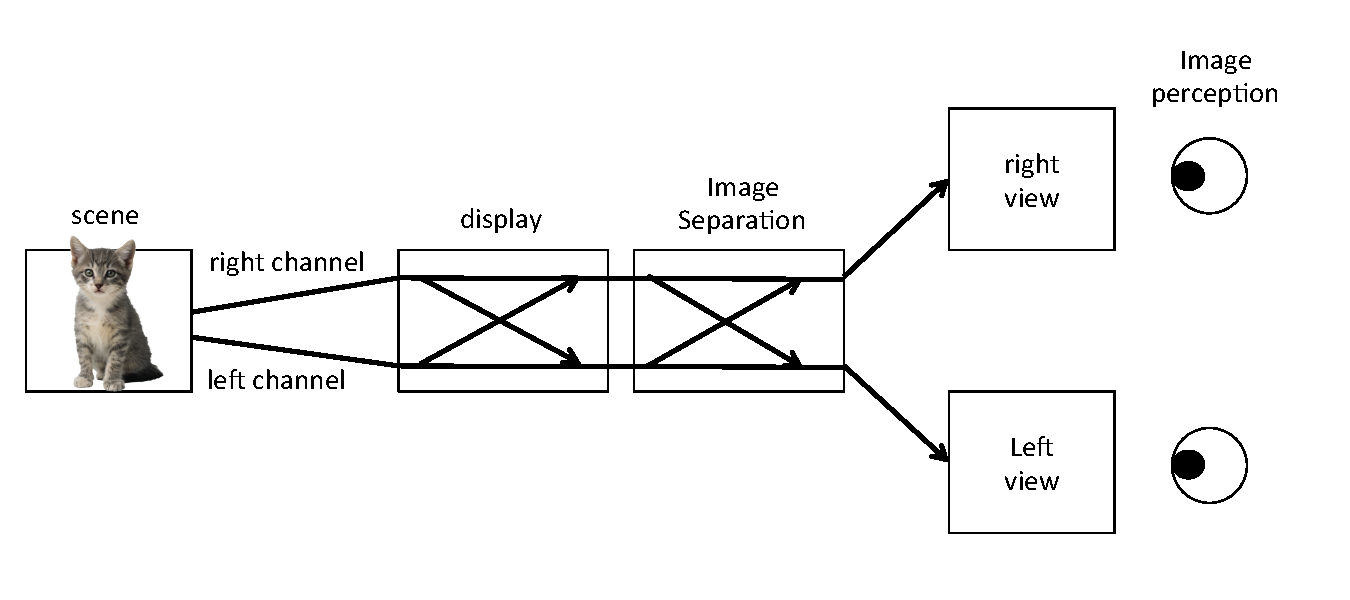
\includegraphics[width=0.9\textwidth]{./Template_Figures/ct_flow}
    \caption{A flow diagram showing the process of stereo image perception starting from stereo scene capture. The crosstalk can be induced by the display (light generation) and by the image/view separation mechanism(3D glasses or autostereoscopic parallax barrier).\label{fig:ctflow}}
\end{figure}

\subsection{Time sequential stereo using active shutter glasses with an LCD display}
LCD screen coupled with active shutter glasses is the most common 3D technology that is commercially available. It produces an image by back lighting a two dimensional individually addressable liquid crystal (LC) \index{LC}matrix. The back light is typically a cold cathode florescent lamp (CCFL) or light emitting diodes (LEDs). The LC matrix consists of crystals that rotate according to the voltage applied to them. This rotation limits the flow of the light that passes through each cell hence producing different gray levels. Each pixel of the screen consists of three LC cells coupled with red, green and a blue filter. Hence the color and luminance of each pixel is created by controlling the light that flows through these individual filters which is regulated by the LCs. It should be noted that even at its best i.e crystals are perpendicular to the light source, they fail to block the light completely and hence an LCD screen can not display true black color.

The time required for the LCs to rotate from one position to another desired position is known as the pixel response rate/time. This response time is higher if the delta between the rotate is smaller and vice versa\cite{woods2012crosstalk}. This means that the refresh rate of an LCD display is dependent upon this response time. LCD displays usually utilize top to bottom image update method i.e. in order to update the image being displayed, the rows of pixels is addressed individually from top to bottom.

\begin{figure}[htbp]
\centering
     \begin{subfigure}[b]{0.4\textwidth}
        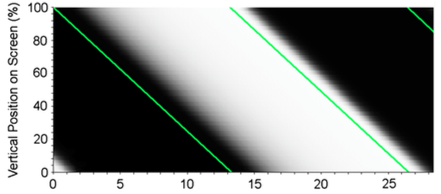
\includegraphics[width=\textwidth]{./Template_Figures/LCD_refresh_low}
        \caption{ Time(ms)}\label{fig:response_low}
    \end{subfigure}
    \begin{subfigure}[b]{0.4\textwidth}
        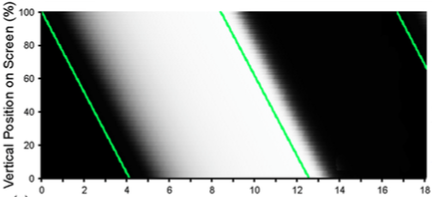
\includegraphics[width=\textwidth]{./Template_Figures/LCD_refresh_high}
        \caption{ Time(ms)}\label{fig:response_high}
    \end{subfigure}

    \caption{\textcolor{red}{(a) Response of a conventional LCD display (in time domain). (b) Response of a high refresh rate LCD display }.  \label{fig:LCD_refresh}}
\end{figure}

figure \ref{fig:LCD_refresh} shows the time domain responses of LCD displays. The green line represents the row of the pixels that are being updated while the images is being changed from complete black to complete white. It case be seen from \ref{fig:response_low} that there is no time (a vertical line) where a complete black or white image is observed. However if the refresh rate is increased (Figure \ref{fig:response_high}), one can see that there is an interval in time where a stable image can be displayed.

Active shutter glasses consists of lenses that can turn opaque or transparent in order to gate the left or right image being displayed on the screen to the respective left or right eye (at any given time, one lens is in opaque state while the other in transparent state). Each lens of these glasses has a liquid crystal called LC shutters(just like an LCD display) that blocks the light when a voltage is applied to it. The time required for these LCs to go from completely opaque to completely transparent and vice versa is called the rise and fall time \cite{woods2012crosstalk}. Figure \textcolor{red}{SHould I use the picture fig 4 from woods?} shows the optical transmission properties of a typical pair of active shutter glasses. It can be seen from this figure that
\begin{figure}
\end{figure}

\begin{itemize}
\item{LC shutters do not perform identically for each wavelength.}
\item{The LC shutters have a non zero transmission even when it is in opaque state.}
\item{The rise and fall time are not instantaneous.}
\end{itemize}

In addition to that, the light transmission in active shutter glasses also varies with the viewing angle. The highest blocking of the light occurs at an angle perpendicular to the shutters. This means that while viewing a scene through these shutter glasses, one would observe grater leakage of light in the border areas of the shutters as compared to the center (provided the position of the eye is in the center of the shutters). It is important that the shutters are opened and closed with the right timings with respect to the image being displayed on the screen. Incorrect image will be observed if the shutters are opened too early or too late that will result in crosstalk.

Hence, the methods according to which crosstalk can occur when using active shutter glasses combined with an LCD display are:
\begin{itemize}
	\item{Optical performance of the liquid crystal cells i.e. crosstalk is proportional to the amount of light leaked while in opaque state.}
	\item{Incorrect synchronization of shutter glasses with respect to the display.}
	\item{Viewing angle through the shutter glasses.}
	\item{Pixel response rate of the LCD display. Higher response time will result in higher crosstalk.}
	\item{Image update method. The ideal time for opening of a shutter would be when an image has been completely displayed on the screen. However most LCDs update the image using vertical scanning and hence usually there is no time at which the image is completely displayed stably.}
	\item{The x,y location of the image on the screen. This is related to both the image update method and the viewing angle through the shutter glasses.}
	\item{The gray level being displayed. If the change in gray level is small then the response time will be large hence causing larger crosstalk. }
\end{itemize}

\subsection{Anaglyph Stereo}
\subsection{Polarized Stereo}
Polarization is a property dealing with the controlled oscillation of light (and other waves). Typically light waves oscillate in a way that their phase shifts over time are unpredictable. Passing the light through special polarizing filters forces them to oscillate in a controlled manner\cite{ wiki:polarizationwiki}. Light can be polarized in a linear manner where the light waves are forced to oscillate in a plane or is a circular manner i.e. the orientation of the oscillations vary circularly with respect to time. In stereoscopy, light intended for the left and right eye can be encoded using linear polarization i.e the polarization of the left eye light is orthogonal to the polarization of the right eye light in case linear polarization is used or the polarization of one view is clockwise and anticlockwise for the other view in case circular polarization is used.

In a typical 3D cinema setup, Images for the left and right eye are simultaneously projected on a silver screen by two projectors. Each of these projectors has a polarizing filter (opposite with respect to each other) attached to it. Viewers view the screen through cheap polarized glasses that has the exact same polarizing filters in its left and right lenses as the left and right projector. This way each of the polarized lens block the light from the other view hence giving an impression of 3D. However, as with every piece of technology, imperfections are also present in this setup. Firstly, the polarizing filters mounted on the projectors are not perfect and fail to properly polarize all light wavelengths and can not be made to be perfectly orthogonal (opposite to each other). \cite{woods2012crosstalk}. Also the silver screen is unable to reflect the polarized light from the projectors without distorting the polarization. Different materials have different polarization properties and up till now a material that perfectly preserves the polarization for all wavelengths has not been discovered. Lastly, it is hard to match the the polarization orientation of the projector filters to the filters present in the glasses. For example, in case of linear polarization, the orientation mismatch can easily occur if the viewers head is slightly tiled hence causing crosstalk \cite{hong2010analysis}. Circular polarization however is less prone to this mismatch as compared to linear polarization hence it is more commonly used in 3D cinemas. In any case, filing to deliver properly polarized left and right image light to the glasses and any mismatch in the orientation of the glasses with respect to the projector filters will hinder the ability of the polarized 3D glasses to block the light from unintended view completely hence causing crosstalk.

In summary, the important factors to consider when dealing with the crosstalk in a typical 3D cinema setup are as follows:
\begin{itemize}
\item{The optical properties of the polarizing filters used in the projectors and the glasses.}
\item{The polarization preserving properties of the screen. }
\item{The mismatch between the orientation of the projection filters with the orientation of the filters present in 3D glasses.}
\end{itemize}

A stereo 3D setup can also be obtained by using a micro-polarized LCD screen used in conjunction with polarized 3D glasses that that similar to the cinema setup discussed above. A micro-polarized LCD screen consists of polarization filters (linear or circular) mounted on top of a conventional LCD screen. However, unlike the projective method where two images can be projected on the screen simultaneously, alternative rows (odd and even rows) of the LCD screen pixels are polarized oppositely to each other. Micro-polarized LCD screens have an advantage over the 3D screens used with active shutter glasses that crosstalk induced due to low refresh rate of the screen is not a problem. But this also comes at a cost of vertical spatial resolution of the the displays as the light from half of the row pixels will be blocked by each of the lens of the polarized glasses. Figure \ref{fig:polarized_lcd} illustrates a typical polarized LCD setup where the user will see different pixel rows in each eye. Figure \ref{fig:polarized_lcd_prob} shows the construction of a typical Polarized LCD screen. It can be seen that the LCD cells are separated from the micro-polarizer film by a glass sheet that is typically 0.5 mm thick \cite{woods2012crosstalk}. Hence a sensitivity to the viewing distance and position due to parallax is induced. This means that if the viewer is not located at the correct position or distance to the screen, he/she will be able to see the unintended rows of pixels along with the intended rows hence inducing crosstalk. In summary, the factors that contribute to the crosstalk in a micro-polarized LCD screen stereo setup are as follows:
\begin{itemize}
\item{Matching of the orientation of the polarization filters in the glasses to the orientation of the micro-polarizing film present on the screen.}
\item{The quality and ability of the micro-polarizing film to properly polarize the light.}
\item{The accuracy of the alignment of micro-polarizing film to the LCD cells.}
\item{x, y screen position of the screen. Due to the fact that viewer will typically be in a position where parallax error mentioned above will vary with the screen position.}
\item{Viewing angle of the viewer as this will affect the matching between the orientation of the glasses and the screen polarization filters.}
\end{itemize}

\begin{figure}[htbp]
\centering
     \begin{subfigure}[b]{0.6\textwidth}
        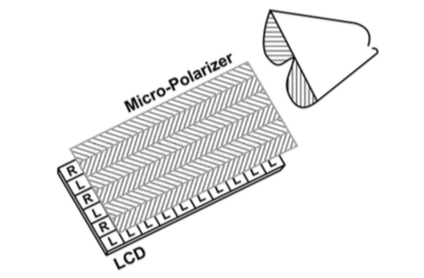
\includegraphics[width=\textwidth]{./Template_Figures/polarized_lcd}
        \caption{ }\label{fig:polarized_lcd}
    \end{subfigure}
    \begin{subfigure}[b]{0.6\textwidth}
        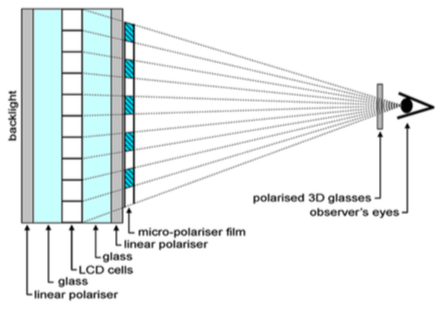
\includegraphics[width=\textwidth]{./Template_Figures/polarized_lcd_problem}
        \caption{ }\label{fig:polarized_lcd_prob}
    \end{subfigure}

    \caption{(a) A layout of a micro-polarized LCD screen where odd and even numbered rows are oppositely polarized. In this example, the viewer viewing the screen using the polarized glasses will see odd numbered pixel rows through the right eye and even numbered pixel rows in the left eye \cite{woods2012crosstalk} (b){Construction of a typical micro-polarized LCD screen}.\label{fig:LCD_refresh}}
\end{figure}

\subsection{Automultiscopic Screens}
discuss lightfeields here as well.

\section{Crosstalk Quality Metrics}

\input{chapters/related_work}


\input{chapters/experiments}
% \input{chapters/model}

%!TEX root = ../Thesis.tex
\chapter{Applications}
\label{chap:applicatons}
In the previous chapters we learned that in addition to viewer's discomfort, reduction of contrast, reduction of stereo acuity, and reduction of overall image aesthetics, crosstalk in stereoscopic screens also has a substantial effect on the observed depth of the disparate objects (i.e., the objects not located at the plane of focus (POF)\index{POF}). The general rule is that the observed depth for any object not lying on the POF will tend to fall back to the POF (losing depth) as the crosstalk level increases, or as the disparity of an object increases. The effect seemed to be more pronounced for objects with narrow width compared to the objects with comparatively wider width, the reason being that the ghost separation (which causes the confusion for HVS) for thin objects is larger for any given disparity. We also learned that, contrary to our intuition, the crosstalk in an automultiscopic screen has little to no effect on the perceived depth for objects of any width for even the most extreme level of crosstalk (14\%). The main reason why crosstalk  did not affect the observed depth might be that in the automultiscopic case, there are two similar ghosts present on each side of the object in both retinal images. This makes the ghost-object combination in both eyes very similar and the HVS might consider them as the same object. Hence, there is nothing to confuse the HVS in estimating the correct disparity between two retinal image patches.

Current literature agree on the theory that the HVS resolves the estimated disparities of objects in a binocular scene by computing the cross-correlation of several patches located at different positions between two perspective retinal images. Finally, we learned that in order to reduce the viewers crosstalk, most of the current state of the art techniques rely upon preprocessing the stereo images in such a way that when, viewed on a stereoscopic or automultiscopic screen, the 
images with system crosstalk added resemble the desired images. Most techniques subtract the pre-calculated light intensity leakage between views from the actual images, and in addition, to using some perceptual measures in order to mask the ghosting that still persists due to the limited dynamic range of the display.

Observed depth reduction due to crosstalk is a serious problem which might alter or degrade the artistic viewing experience for a scene. Similar to we have image quality metrics e.g. SSIM \cite{wang2004image}, MSE\cite{ wiki:MSE} or VDP\cite{mantiuk2004visible} used to calculate the effects of noise in an image on its perception by a human observer as compared to the noise-free images, it would be useful to have a quality metric that is able to predict the observed depth of objects of interest in a 3D scene based on the crosstalk level of the display along with the dimensions and disparity of the object. Once this prediction is available, the scene artists can then alter the theoretical depths of the objects in order to bring the observed depths as close to the desired depth as possible. For this to work, however, we should have a good understanding of how the HVS estimates the depth from disparity between two retinal images, and hence derive an accurate HVS model. Moreover, reducing the viewer's crosstalk for any given display is also as important if not more for a better viewing experience. The most promising techniques to achieve that use complex optimizations to be performed in order to pre-process the images\cite{van2011perceptually}. It would be helpful if similar effects can be achieved without the mentioned complex and time consuming optimizations.

In this chapter, we will look into a proposed modified HVS depth from disparity resolution model that provides a good initial approximation to the observed depths obtained from our experiment results discussed in the previous chapter. We will also propose two new crosstalk reduction techniques along with there advantages and disadvantages and their results.

\section{Observed depth prediction}

Filippini et al \cite{filippini2009limits} proposed a model that simulated the depth estimation of the HVS via disparity. In short, this model computes the local cross-correlation that is defined by Eq \ref{eq:banks_ccr}.
\begin{equation}
c(\delta_x) = \frac{ \sum\limits_{(x,y) \in W_L} [(L(x,y) - \mu_L)(R(x-\delta_x, y) - \mu_R)] }{\sqrt{\sum\limits_{(x,y) \in W_L}(L(x,y) - \mu_L)^2} \sqrt{\sum\limits_{(x,y) \in W_R}(R(x-\delta_x, y)- \mu_R)^2}},
\label{eq:banks_ccr}
\end{equation}
where
\begin{equation}
W_L \:=\: W_R \:=\: e^{-\left(\frac{x^2}{2\sigma_x^2} \:+\: \frac{y^2}{2\sigma_y^2}\right)}
\label{ccr_windows}
\end{equation}
are anisotropic Gaussian windows (patches) in the left and the right stereo images. The window $W_L$ is fixed in one image while $W_R$ is displaced horizontally while keeping the vertical position constant. For each displacement $\delta_x$, $c(\delta_x)$ is computed resulting in a value in the range [-1,1] (1 if the patches are perfectly correlated, -1 if the patches have no correlation at all). The value of $\delta_x$ for which the maximum cross-correlation is attained is considered to be the disparity of the pixel (centered at the window) in the right image w.r.t the left image. The process is repeated for all the pixels in the left image. The depth estimates using this model, and the human observed depths of the peaks and troughs in random dot stereogram consisting of saw-toothed corrugations of different frequencies and amplitudes were compared by the authors. They found that in addition to their estimated depths matching closely with the viewer's observed depths, their model also correctly estimated the HVS's threshold (for distinguishing between disparities) for the upper and lower spatio-temporal frequencies. However, the random dot stereograms used were devoid of any crosstalk.

We tested the same model on our stimuli (Chapter 4) and found that this model always resulted in the correct disparity of the objects between a stereo image pair. That is, the crosstalk had no effect on the disparity the disparity estimated by the model. This did not match the results we obtained in our experiments with the human observers. The reason is that even though the areas on the images where the ghosts are present will show some positive correlation, the maximum correlation is always obtained at the location where the actual object is located.

Hence it is clear that the HVS does not simply estimate the depth from disparity as the maximum of local cross-correlation only. It is believed that the HVS, while matching patches between retinal images, prefers lower disparity over higher ones \cite{howard1995binocular}. This means that, for any patch in e.g. the left eye retinal image, if the HVS finds two matching patches in the right image, it will choose the one that is closest to the location of the left image patch. Recall from the previous chapter that in the case of stereo displays with some level of crosstalk, for a disparate object in the the left image, the same object is located at some horizontal disparity \emph{d} where as the ghost is located exactly at zero disparity (same location as the location of the object in the left image). Computing a cross-correlation in this case would result in some positive correlation because of the ghost at zero disparity and a highly positive correlation at disparity \emph{d}. To match the results from human observers, the disparity estimator model should have the following characteristics:
\begin{itemize}
\item{Select a disparity \emph{d} based local cross-correlation.}
\item{In the presence of crosstalk, estimated disparity \emph{d} should shift towards zero disparity gradually as the actual disparity increases over some threshold.}
\item{Estimated disparity should be estimated as 0 if the crosstalk level increases over some threshold (e.g. more than 14\%) or if the disparity is above some level (exceeding Panum's fusion area \footnote{Panum's fusion area is the space around the POF where single binocular vision is observed. Double vision (diplopia) is observed for objects outside the Panum's fusion area.}).}
\end{itemize}
Hence we may assume that the model should somehow weigh the resulting cross-correlation profile prior to obtaining the disparity estimate. We observe that weighing the cross-correlation profile with a Gaussian function centered at the location of ghost in the left eye image fulfills the aforementioned requirements. This can be seen in Fig \ref{fig:windowed_ccr_f}.
\begin{figure}[htbp]
    \centering
    \begin{subfigure}[b]{0.9\textwidth}
        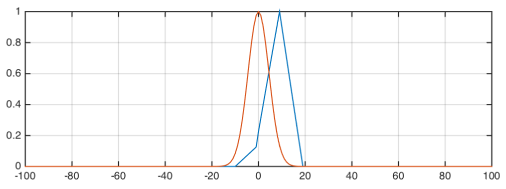
\includegraphics[width=\textwidth]{./Template_Figures/normal_ccr}
        \caption{}\label{fig:normal_ccr}
    \end{subfigure}

    \begin{subfigure}[b]{0.9\textwidth}
        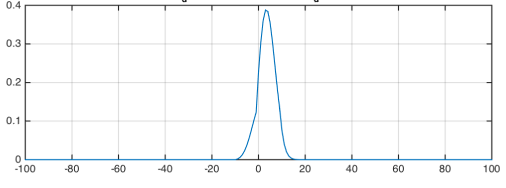
\includegraphics[width=\textwidth]{./Template_Figures/windowed_ccr}
        \caption{}\label{fig:windowed_ccr}
    \end{subfigure}

    \caption{The figure represents estimating the human observed disparity in a thin cylinder stereo pair where the disparity in terms of pixels is 9 and the crosstalk is 14\%. The cross-correlation of a patch containing only the cylinder from the right eye image is computed across the entire left eye image containing both the cylinder and the ghost. (A) The blue line represents the 1D The scan line of the result of local cross-correlation. In this case, the maximum cross-correlation occurs at the disparity of 9 pixels, which is the actual disparity. Orange line represents a Gaussian function with $\sigma$ = 9 pixels centered at the location of the ghost that is to be used for weighing the correlation profile. (B) The resulting Gaussian weighed local cross-correlation. It can be seen that, the estimated disparity as a result of the peak of cross-correlation has shifted back from 9 to 3 pixels.\label{fig:windowed_ccr_f}}
\end{figure}

In our disparity estimation model, we assume that the HVS will be able to isolate the object of interest in one (source) retinal image (due to its luminance profile) and try to find an appropriate match for that object in the other target image. The target image has of two possible matches i.e. the ghost and the object itself. For simplicity, we show the resulting cross-correlation for a single scan line of the stereo image pair. This is sufficient to estimate the disparity of s single fixed width object. Figure \ref{fig:normal_ccr} (blue line) represents the cross-correlation profile for a cylinder that has a width of 9 pixels and is located at the disparity of 9 pixel. The background for simplicity in this case is black. We can see that there is some positive correlation at zero disparity due to the 14\% crosstalk induced ghost. However, the full correlation (+1) is attained at the disparity 9, indicating the actual disparity of the object. The orange line represents how the resulting correlation profile is weighted by a truncated Gaussian that has a standard deviation of 9 pixels. The Gaussian weighed correlation profile in Figure \ref{fig:windowed_ccr} is obtained by simple point-wise multiplication of the two functions in Figure \ref{fig:normal_ccr}. It can be seen that after weighing with the Gaussian window for which the standard deviation $\sigma$ is roughly equal to the width of the object, the maximum correlation occurs at a disparity of 3 pixels. This means that, the perceived depth via disparity would be approximately 3 pixels (around 1.18 cm). So, in this, case the estimated disparity is quite close to the result that we obtained from the experiments.

\begin{figure}[H]
\centering
    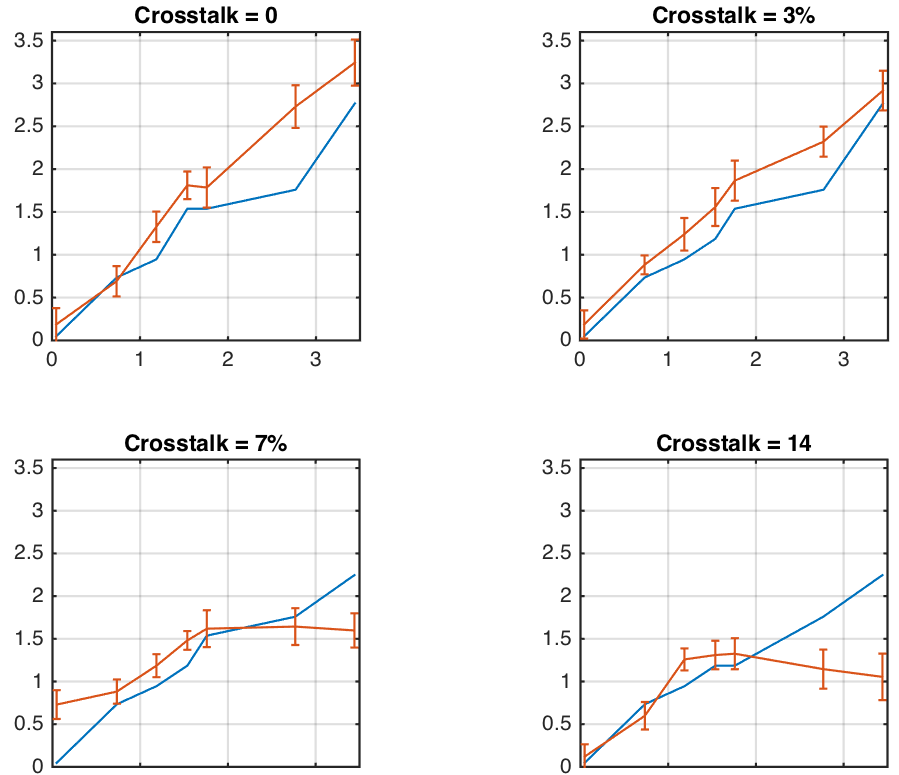
\includegraphics[width=0.7\textwidth]{./Template_Figures/s_9_sigma_7_4}
    \caption{Comparison of experimental observed depth for cylinder of 18.9 arc min width (orange) vs estimated depth via windowed cross-correlation. The best results were obtained with $\sigma$ = 15.4 arc min.\label{fig:s_9_sigma_7_4}}
\end{figure}
\begin{figure}[H]
\centering
    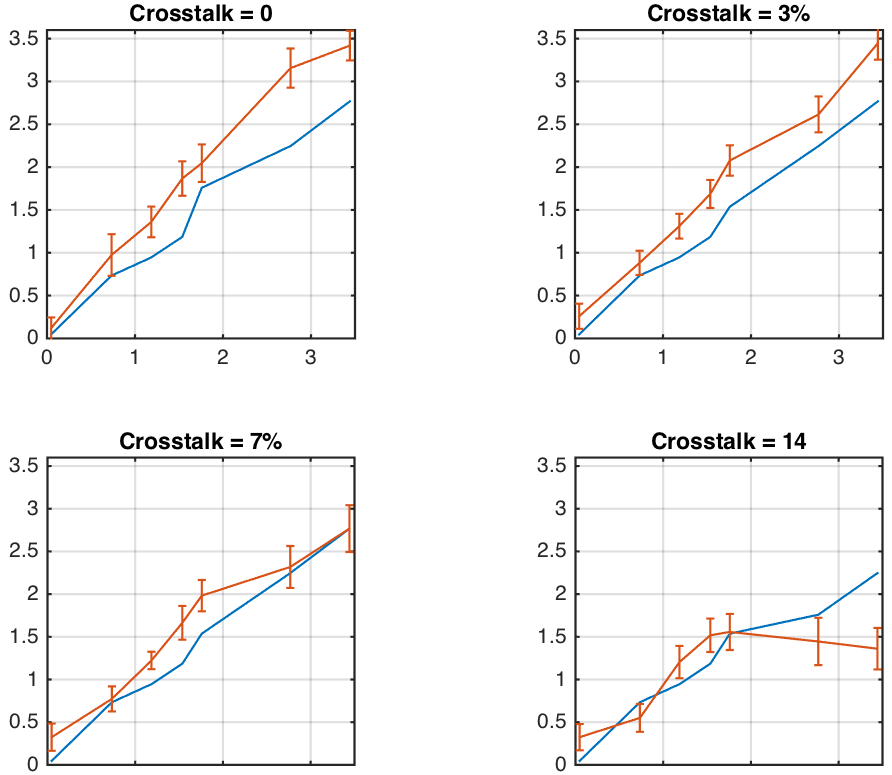
\includegraphics[width=0.7\textwidth]{./Template_Figures/s_18_sigma_14_7}
    \caption{Comparison of experimental observed depth for cylinder of 37.8 arc min width (orange) vs estimated depth via windowed cross-correlation. The best results were obtained with $\sigma$ = 30.87 arc min.\label{fig:s_18_sigma_14_7}}
\end{figure}
\begin{figure}[H]
\centering
    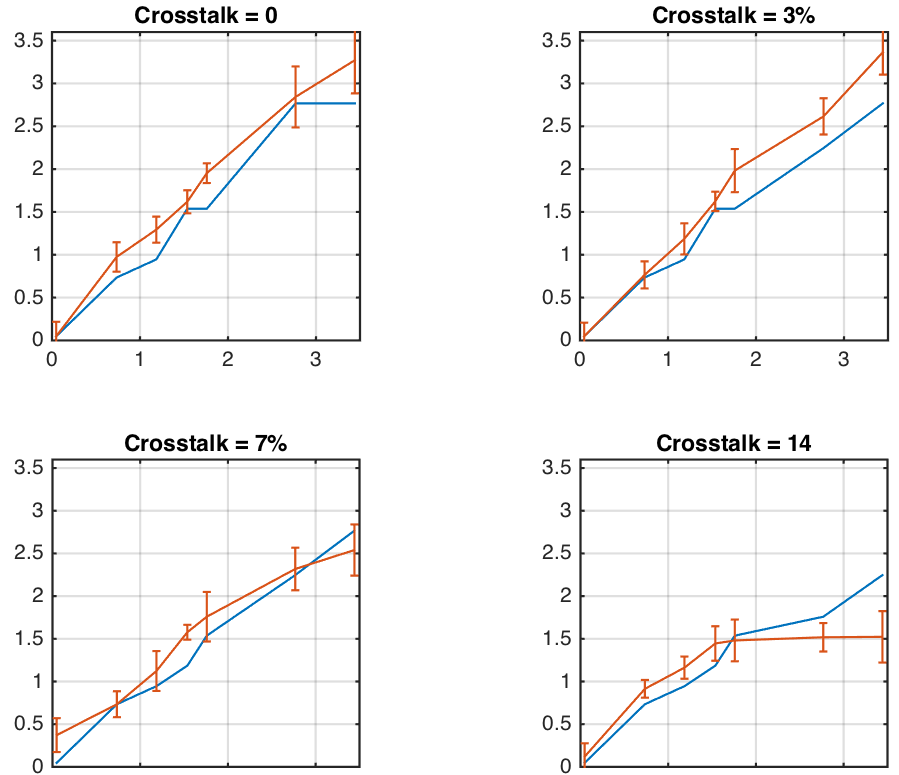
\includegraphics[width=0.7\textwidth]{./Template_Figures/s_27_sigma_17_4}
    \caption{Comparison of experimental observed depth for cylinder of 56.7 arc min width (orange) vs estimated depth via windowed cross-correlation. The best results were obtained with $\sigma$ = 36.54 arc min.\label{fig:s_27_sigma_17_4}}
\end{figure}
\begin{figure}[H]
\centering
    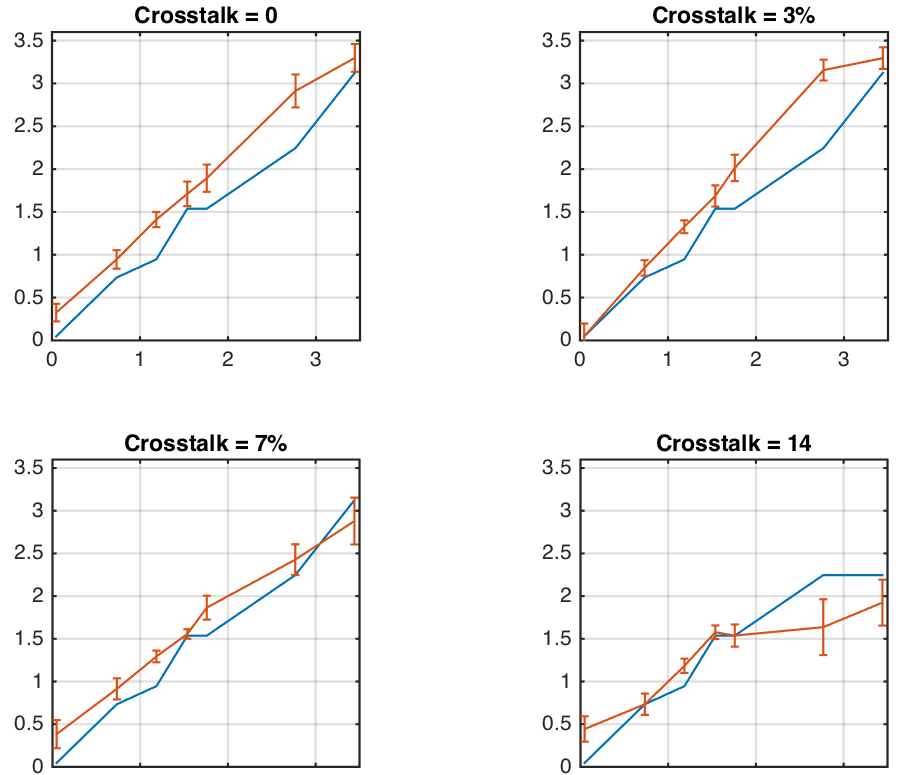
\includegraphics[width=0.7\textwidth]{./Template_Figures/s_36_sigma_22}
    \caption{Comparison of experimental observed depth for cylinder of 75.6 arc min width (orange) vs estimated depth via windowed cross-correlation. The best results were obtained with $\sigma$ = 46.2 arc min.\label{fig:s_36_sigma_22}}
\end{figure}

We simulated our stereo experiments for the cylinders and computed the estimated depths using our Gaussian weighted cross-correlation model. Figure \ref{fig:s_9_sigma_7_4} to Figure \ref{fig:s_36_sigma_22} shows the results that we obtained and there comparison with the data we got from our experiments. We observed that even thought this model had some short comings and did not fit to all of the data properly, it was able to mimic the degradation of estimated depth as the crosstalk level or the disparity increased. The figures above represent the estimated depths using a our Gaussian weighed local cross-correlation model with fixed $\sigma$ for each cylinder that best matched the data. For almost all the cases (specific disparities and crosstalk levels) where the estimated depth was incorrectly estimated, we were able get approximately matching results using some $\sigma$. However, we were not able to find one $\sigma$ that matched all cases for a particular cylinder. Perhaps the HVS weighs the cross-correlation profile with Gaussians of different standard deviations for different object widths and disparities. Our Gaussian window-weighted local cross-correlation model has the advantage that it resolves to a degraded estimated depth in the case where certain level of crosstalk is present. However, the short coming is that it also, to some extent, penalizes the estimated depth even if there is no crosstalk present. This does not conform fully to our experimental data. However, it may gives the right direction for the future research in this area.
\pagebreak

\section{Crosstalk mitigation}

During the course of this thesis, we devised and tested some new ideas to improve the current crosstalk reduction techniques. In this section we review those ideas.

\subsection{Unsharp masking in epipolar domain}
The Corn-sweet illusion \cite{ wiki:cornsweet} is used in contrast boosting image processing techniques such as unsharp masking. The basic idea of unsharp masking is to add to an image a high frequency image of itself. The high frequencies containing image is obtained by subtracting a blurred version of the image from itself. Baar et al \cite{van2011perceptually} used a similar technique to blur the uncorrectable crosstalk in combination with increasing the contrast of the objects around the edges. One can generally use unsharp masking to increase the contrast of an image suffering from contrast loss due to preprocessing for crosstalk compensation . However applying unsharp masking in spatial domain also boosts the unwanted noise. Since automultiscopic screens displays lightfields, and given the fact that crosstalk in any perticular view in induced by the neighboring views, intuitively, it would make sense to applying unsharp masking in the view domain (also called as the epipolar domain) that would result in a crosstalk compensated lightfield with increased local contrast around the object. Let $\Psi$ be a lightfield in which x, y denote the spacial dimensions on the displayed image and w denotes the epipolar domain (Figure \ref{fig:lightfeild})
\begin{figure}[htbp]
    \centering
    \begin{subfigure}[b]{0.48\textwidth}
        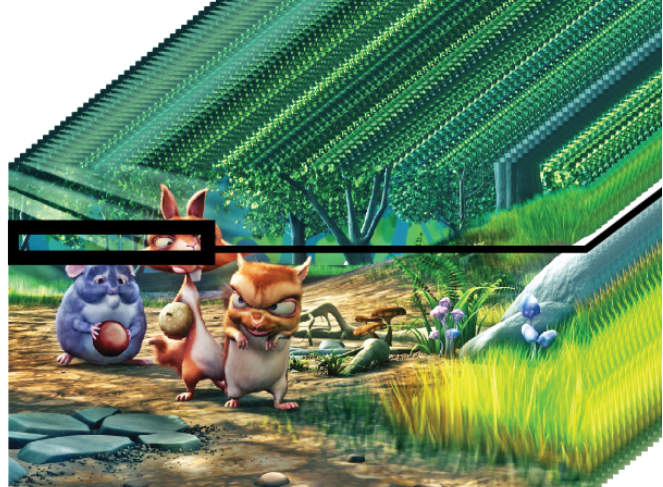
\includegraphics[width=\textwidth]{./Template_Figures/lightfield}
        \caption{}\label{fig:lightfield_rep}
    \end{subfigure}
    \begin{subfigure}[b]{0.48\textwidth}
        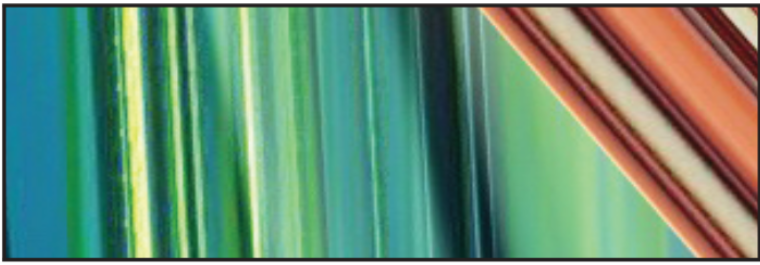
\includegraphics[width=\textwidth]{./Template_Figures/lightfield_epi}
        \caption{}\label{fig:lightfield_epi}
    \end{subfigure}

    \caption{Representation of a 3D lightfield \cite{du2014improving}. (A)(\emph{x,y}) denotes the view dimensions while \emph{w} denotes different perspective views for a light field. (B) Epipolar view of the squared region in (a)representing how every pixels shifts with respect to shift in perspective.\label{fig:lightfeild}}
\end{figure}
\pagebreak

\noindent 
Then for an automultiscopic screen where only the light from the immediate neighbors is leaked, we blur the lightfield in epipolar domain with the following 1D kernel:
\begin{table}[H]
\centering
\begin{tabular}{|c|c|c|}
\hline
$\omega_1$ & $\omega_2$ & $\omega_3$ \\
\hline
\end{tabular}
\label{tab:blurring_kernel}
\end{table}
\noindent
This will result in a epipolar domain blurred light field $\Psi_{blr}$. Next we subtract $\Psi_{blr}$ from the original light field $\Psi$. This will give us  $\Psi_{hf}$, a light field that only contains luminance-inverted ghosts in every view. i.e.
\begin{equation}
\Psi_{hf}\: =\: \Psi\: -\: \Psi_{blr}
\end{equation}
The crosstalk-compensated light field is obtained as
\begin{equation}
\Psi_{opt}\: =\: \Psi\: +\: \Psi_{hf}
\end{equation}
Hence, for every view image $I \in\: \Psi_{opt}$
\begin{equation}
\begin{aligned}
I_{opt}\: =\:  I + (I - \omega_1I_L - \omega_2I - \omega_3I_R) \\
I_{opt}\: = \: (2-\omega_2)\ I\: -\: \omega_1I_L\: -\: \omega_3I_R
\end{aligned}
\end{equation}
Where $I$ is the view centered image and $I_L, I_R$ are the immediate left and right neighbors respectively. Since the automultiscopic screen will display the optimized light field image as a weighted sum of $I_L, I_R$ and $I$ i.e.
\begin{equation}
\begin{aligned}
I_{observed}\: =\:  \Phi_1.I_{L(opt)}\: + \:\Phi_2.I_{(opt)}\: + \:\Phi_3.I_{R(opt)}       \\
I_{observed}\: = \: \Phi_1{(2-\omega_2) I_L\: -\: \omega_1I_{LL}\: -\: \omega_3I}\:+  \\
                    \Phi_2{(2-\omega_2) I\: -\: \omega_1I_{L}\: -\: \omega_3I_R}\:+   \\
                    \Phi_3{(2-\omega_2) I_R\: -\: \omega_1I\: -\: \omega_3I_{RR}}
\end{aligned}
\end{equation}
Here $I_{LL}$ and $I_{RR}$ are the immediate left and right images to left and right image of the view position in the light field. We know, from view-luminance intensity profiles for an automultiscopic screen \ref{fig:sim_gaussians}, that:
\begin{equation}
\begin{aligned}
\Phi_1\:=\: \Phi_3\:=\: 0.0351,\:\: \Phi_2\:=\:0.8
\end{aligned}
\end{equation}
In order to cancel the effect of $I_L$ and $I_R$ for crosstalk compensation, we choose
\begin{equation}
\begin{aligned}
\omega_1\:=\: \omega_3\:=\: 0.0421,\:\: \omega_2\:=\:1.19
\end{aligned}
\end{equation}
Using the aforementioned values of $\omega_1$, $\omega_2$, $\omega_3$, $\Phi_1$, $\Phi_2$ and $\Phi_3$, the viewer observed image $I_{observed}$ can then be mathematically written as
\begin{equation}
I_{observed}\: =\:  1.42.I\:-\: 0.0014(I_{LL}\:+\:I_{RR})
\label{eq:final_unsharp_obs}
\end{equation}

It can be seen from Equation \ref{eq:final_unsharp_obs} that even though the crosstalk effect induced by the immediate left and right image of a view has been eliminated. However, some over-subtraction of luminance due to the $I_{LL}$ and $I_{RR}$ propagates in the observed image $I_{observed}$. Even though compensating for crosstalk in this manner is quite efficient, one can see the average luminance of the view centered image $I$ has been increased to 1.42. Since the maximum luminance value an automultiscopic screen can display is 1, our proposed technique will result in clipping of the all the luminance values above 1 hence resulting in loss of contrast. Another drawback, as describbed in Figure \ref{fig:why_no_cornsweet}, unsharp masking in view domain of a light field does not introduce any Cornsweet profiles.

\begin{figure}[htbp]
    \centering
    \begin{subfigure}[b]{0.48\textwidth}
        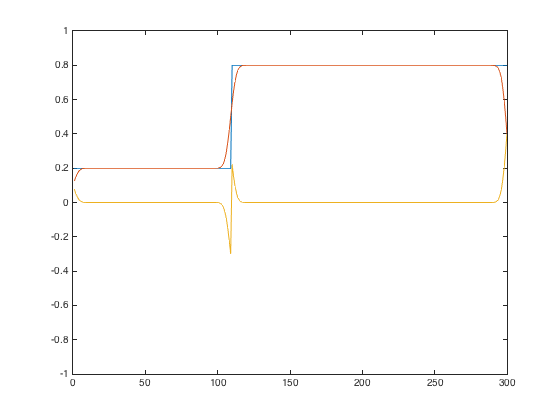
\includegraphics[width=\textwidth]{./Template_Figures/unsharp_proper}
        \caption{}\label{fig:cornsweet}
    \end{subfigure}
    \begin{subfigure}[b]{0.48\textwidth}
        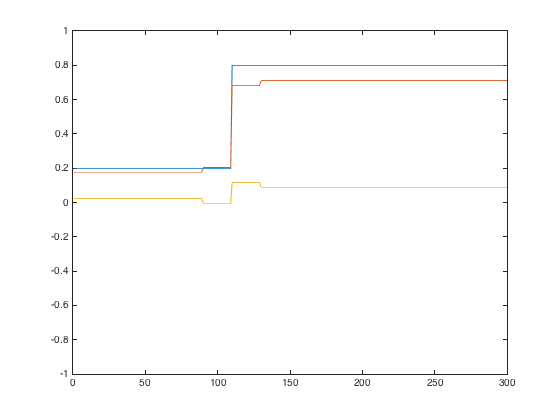
\includegraphics[width=\textwidth]{./Template_Figures/unsharp_epipolar}
        \caption{}\label{fig:no_cornsweet}
    \end{subfigure}

    \caption{(A) 1D representation of luminance profile along an image row. Blue graph represents a luminance step and orange graph represents the luminance profile of the blurred image. Yellow graph represents corn-sweet profile centered at the luminance edge and obtained as the difference between the original and the blurred image.  (B) Same procedure performed in view domain. Blue graph represents the luminance profile of a light feild image and orange graph represents the non-energy preserving additive blurring due to neighboring views in an automultiscopic environment. The Yellow graph represents the difference between the view image and its view-domain blurred version that resembles closely to subtractive crosstalk cancellation rather than a corn-sweet profile.\label{fig:why_no_cornsweet}}
\end{figure}

\subsection{Iterative crosstalk reduction}

To the best of our knowledge, all the current subtractive crosstalk reduction techniques compute the pre-processed crosstalk compensated images by subtracting the amount of leaked light between neighboring views. The calculation of subtracted leaked light is always performed while considering the unmodified stereo image pair. We observe that the amount of light leaked into a view image due to the unmodified alternative view image should be different when the alternate view image is already crosstalk compensated. This is the case in reality and hence we think that a view image should be compensated appropriately if it alternative view image is already crosstalk compensated. Inspired by this idea, we propose an iterative subtractive crosstalk reduction technique.

Consider a light field $\Psi$ consisting of a set of view images ${f_1, f_2, ..., f_N}$. When the $i^{th}$ view is displayed on an automultiscopic screen, its crosstalk $\phi(f_i)$ from the neighboring views can be written as
\begin{equation}
\phi(f_i)\:=\: a_1.f_1\:+\:a_2.f_2\:+\:...\:a_{i-1}.f_{i-1}\:+\:a_{i+1}.f_{i+1}\:+\:...\:a_n.f_n
\end{equation}
Where the light intensity leakage values $a_1...a_n$ are given by the curves in Figure \ref{fig:sim_gaussians}. The crosstalk compensated images $\{\gamma_1...\gamma_n\}$ can then be computed iteratively as:
\begin{equation}
\begin{aligned}
\gamma_1^{n+1} \:=\: f_1 \:+\: \phi(\gamma_1^n) \\
\gamma_2^{n+1} \:=\: f_2 \:+\: \phi(\gamma_2^n) \\
.\:\:\:\:\:\:\:\:\:\:\:\:\:\:\:\:\:\:\:\:\:\:\:\:\:\:\:\:\:\:\:\:\:\:\:\:\:\ \\
.\:\:\:\:\:\:\:\:\:\:\:\:\:\:\:\:\:\:\:\:\:\:\:\:\:\:\:\:\:\:\:\:\:\:\:\:\:\ \\
.\:\:\:\:\:\:\:\:\:\:\:\:\:\:\:\:\:\:\:\:\:\:\:\:\:\:\:\:\:\:\:\:\:\:\:\:\:\ \\
\gamma_N^{n+1} \:=\: f_N \:+\: \phi(\gamma_N^n) \\
\end{aligned}
\end{equation}
Where \emph{n} is the number of current iteration. After each iteration, clipping of the values exceeding the display's dynamic range is performed. The iterations terminate when the error $\epsilon$ falls below a threshold.
\begin{equation}
\begin{aligned}
\epsilon \:=\: \sqrt{(\gamma_1^{n+1}\:-\:\gamma_1^n)^2 \:+\: ...\:+\:(\gamma_N^{n+1}\:-\:\gamma_N^n)^2}
\end{aligned}
\end{equation}

This technique compensates for the crosstalk more appropriately. However, the successive subtraction of luminance from the light field view images between iterations might result in lower average luminance in the crosstalk compensated light field (Figure \ref{fig:iterative_tech}).
\begin{figure}[htbp]
    \centering
    \begin{subfigure}[b]{0.48\textwidth}
        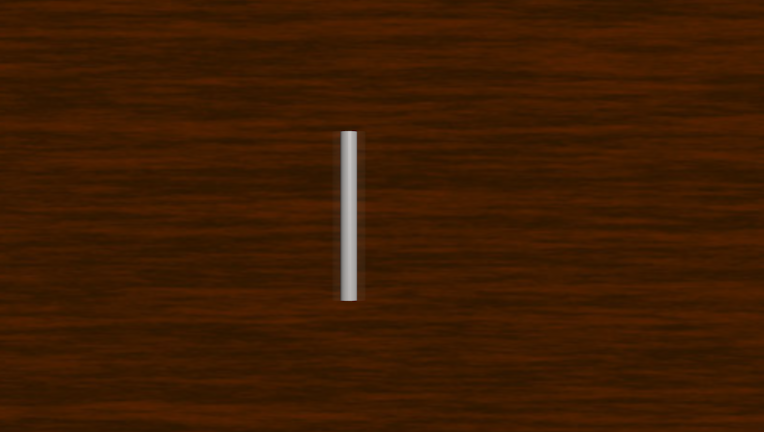
\includegraphics[width=\textwidth]{./Template_Figures/image_w_ct}
        \caption{}\label{fig:original_lf}
    \end{subfigure}

    \begin{subfigure}[b]{0.48\textwidth}
        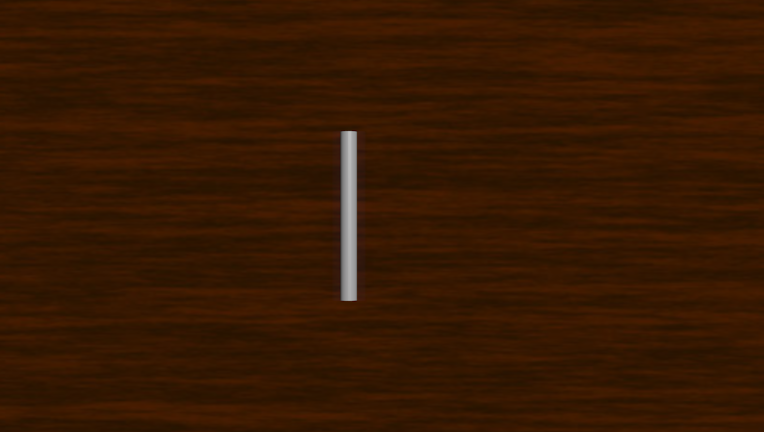
\includegraphics[width=\textwidth]{./Template_Figures/subtractive_comp}
        \caption{}\label{fig:subtractive_lf}
    \end{subfigure}
    \begin{subfigure}[b]{0.48\textwidth}
        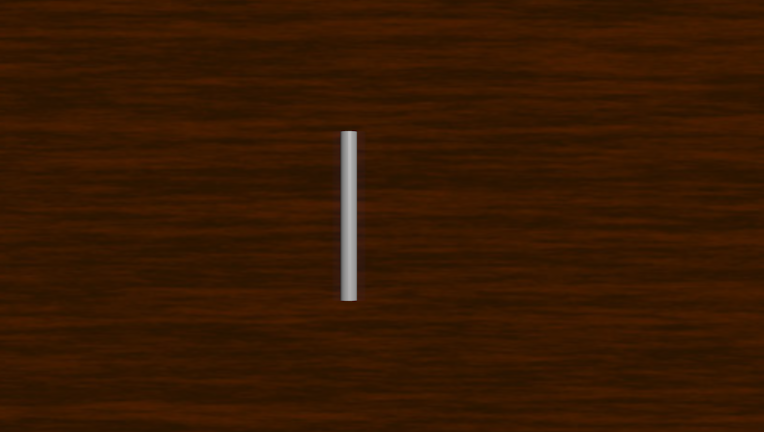
\includegraphics[width=\textwidth]{./Template_Figures/iterative_comp}
        \caption{}\label{fig:iterative_lf}
    \end{subfigure}

    \caption{Naive subtractive crosstalk compensation compared to our proposed iterative crosstalk compensation. (A) An automultiscopic display's view image containing crosstalk given by the curves in Figure \ref{fig:sim_gaussians}. (B) Compensated view image using naive crosstalk subtraction. (C) Compensated view image using iterative crosstalk subtraction. \label{fig:iterative_tech}}
\end{figure}


% \subsection{Proposed optimizations}
% \subsection{Unsharp masking in view domain}
% \subsection{Iterative subtraction}


%!TEX root = ../Thesis.tex
\chapter{Conclusion}

\section{Summary}

\section{Future Work}

\section{Open Questions}


% *************** Bibliography ***************
\bibliographystyle{acm}
{\small\bibliography{bibliography/references}}
\clearpage

% *************** Appendixes ***************
\addtocontents{toc}{\vspace{2em}}
\appendix
%\appendixpage*


% ****************** Index *******************
\printindex

% *************** Back matter ***************
%\backmatter
%\input{back.tex}

\end{document}